\documentclass[11pt,a4paper]{article}
\usepackage{fontspec}
\setmainfont{Noto Serif}
\setsansfont{Noto Sans}
\setmonofont{Noto Sans Mono}[Scale=0.86]
\usepackage[english]{babel}
\usepackage{amsmath,amssymb,amsthm,mathtools}
\usepackage{geometry,booktabs,longtable,tabularx,array,graphicx}
\usepackage{xcolor,hyperref,xurl,fancyhdr,enumitem}
\geometry{margin=2.2cm,headheight=15pt}
\definecolor{ink}{HTML}{183449}
\definecolor{teal}{HTML}{187C80}
\hypersetup{colorlinks=true,linkcolor=ink,citecolor=teal,urlcolor=teal,
pdftitle={ECDR: HAPT Data Analysis and Methodological Implications},pdfauthor={ECDR Research}}
\urlstyle{same}
\setlength{\parindent}{0pt}
\setlength{\parskip}{5pt}
\setlength{\emergencystretch}{3em}
\setlength{\tabcolsep}{4pt}
\renewcommand{\arraystretch}{1.16}
\setlist{nosep,leftmargin=1.5em}
\newcolumntype{Y}{>{\raggedright\arraybackslash}X}
\newcolumntype{P}[1]{>{\raggedright\arraybackslash}p{#1}}
\newcommand{\R}{\mathbb R}
\newcommand{\norm}[1]{\left\lVert#1\right\rVert}
\newcommand{\abs}[1]{\left\lvert#1\right\rvert}
\newcommand{\code}[1]{{\small\ttfamily\nolinkurl{#1}}}
\newcommand{\ind}{\mathbf1}
\newtheorem{proposition}{Proposition}[section]
\newtheorem{lemma}[proposition]{Lemma}
\theoremstyle{definition}
\newtheorem{definition}[proposition]{Definition}
\newtheorem{example}[proposition]{Example}
\newtheorem{remark}[proposition]{Remark}
\renewcommand{\proofname}{Proof}
\pagestyle{fancy}
\fancyhf{}
\fancyhead[L]{\small\textcolor{ink}{ECDR | Data Foundations and Analysis}}
\fancyhead[R]{\small HAPT Dataset and Decision Reuse Methodology}
\fancyfoot[L]{\small October 2026 | English Research Edition}
\fancyfoot[R]{\thepage}
\begin{document}
\hypersetup{pageanchor=false}
\begin{titlepage}
\vspace*{1.0cm}
{\Large\color{teal} THEORETICAL RESEARCH -- SPECIAL TOPIC REPORT\par}
\vspace{0.6cm}
{\huge\bfseries\color{ink} Empirical Analysis of the HAPT Dataset\\and Methodological Implications for ECDR\par}
\vspace{0.7cm}
{\Large From Physical Measurements, Annotations, and Window Geometry\\to Perturbation Domains and Certified Decision Reuse Protocols\par}
\vspace{1cm}
\begin{tabularx}{\linewidth}{@{}P{3.2cm}Y@{}}\toprule
Role & Dedicated technical companion extending Week~2 and the foundational Week~1--3 theoretical report.\\
Scope & All 61 raw sensor recording pairs, 1,214 annotation spans, 17,453 sliding windows, and disjoint subject split metadata in the workspace.\\
Methodology & Exhaustive raw audit, descriptive and geometric statistics, coordinate-level verification, and rigorous combinatorial derivations.\\
Boundaries & Read-only data audit; no CNN model training or inference is performed; proximity in sensor space is never conflated with mathematical decision certification.\\
Reproducibility & Fully automated via \code{qa/data_cnn/prepare_data_analysis.py} and audited via \code{qa/data_cnn/data_analysis.json} under directory \code{me}.\\\bottomrule
\end{tabularx}
\vfill
\textbf{Central Findings.} Sensor streams exhibit strong local temporal continuity and exact sample-sharing across consecutive sliding windows upon temporal alignment. However, the same-coordinate positional distance between adjacent windows possesses a heavy-tailed distribution that varies by orders of magnitude across physical activities. Crucially, the standard sliding window policy severely degrades support for brief postural transitions due to stride-grid phase misalignment. Consequently, safe and beneficial Event-Conditioned Decision Reuse (ECDR) cannot rely on a naive global distance threshold or raw sample proximity. Instead, reuse domains must combine structured temporal dynamics with formal classifier output certificates evaluated under transparent, stream-level denominators.
\end{titlepage}
\hypersetup{pageanchor=true}
\pagenumbering{arabic}

\section*{Executive Summary}
\addcontentsline{toc}{section}{Executive Summary}
This audit inspects all 1,122,772 raw time samples collected across 30 human subjects in the UCI Smartphone-Based Recognition of Human Activities and Postural Transitions (HAPT) dataset. Each raw sample comprises six tri-axial sensor channels (3-axis accelerometer and 3-axis gyroscope), producing exactly 6,736,632 physical sensor coordinates. Applying the standard temporal windowing configuration ($W=128$ samples, stride $S=64$ samples at 50~Hz) yields 17,453 multivariate window inputs of dimension $6 \times 128$. An exhaustive coordinate-level audit confirms that all 13,403,904 coordinates in the saved window tensor exactly reproduce the raw text source under single-precision float conversion (zero mismatch). Furthermore, all 6,678,528 overlapping coordinates across the 17,392 temporally adjacent window pairs match identically upon shift alignment.

These checks establish data integrity and numerical reproducibility. However, they do not validate physical calibration, semantic annotation indexing, classifier accuracy, or certification soundness. Those critical boundaries are rigorously isolated in this report.

Among the 10,361 pure-label windows, only 344 belong to the six postural transition classes. The class \code{SIT_TO_STAND} retains only 12 pure windows across the entire dataset, containing zero adjacent pure pairs. We prove that this empirical collapse is a mathematical consequence of the windowing grid: 40 annotation spans are strictly shorter than 128 samples ($<2.56$~s), while another 91 spans are sufficiently long but contain no window that aligns with the stride-64 lattice. This is an artifact of the discretization pipeline rather than an indicator that postural transitions are unimportant for downstream applications.

Distance analysis in a dimensionless coordinate system (normalized via pure 6-class training windows) reveals that while the median normalized $L_2$ distance between adjacent pure windows of the same class is 4.94, its 90th percentile reaches 46.42. More importantly, static postures (sitting, standing, laying) exhibit median adjacent distances of $1.09 - 1.76$, whereas dynamic locomotion activities (walking, walking upstairs, walking downstairs) exhibit medians of $32.86 - 44.87$. Consequently, any single global perturbation threshold is fundamentally ill-suited for decision reuse. No empirical threshold in this report is endorsed as an off-the-shelf reuse certificate without formal verification.

\begingroup\small\setlength{\parskip}{0pt}\tableofcontents\endgroup
\clearpage

\section{Research Questions and Evidence Standards}

\subsection{Why Must Data Be Analyzed Before CNNs and Certification?}
Event-Conditioned Decision Reuse (ECDR) monitors an incoming stream of multivariate sensory inputs $X_0, X_1, \ldots$ and seeks to reuse the classification decision of a reference neural network $f_\theta$ whenever it can be certified that the decision remains invariant. The data stream determines what inputs the model receives, the geometric relationship between consecutive model queries, the meaningful shape of perturbation domains, and which cases enter the denominator of reuse coverage.

If the empirical unit of observation is misunderstood, or if challenging stream segments (such as boundary-crossing or ambiguous windows) are filtered out prior to measurement, an apparently high reuse rate may merely reflect an artificially benign denominator.

This report addresses six interdependent questions:
\begin{enumerate}[label=\textbf{(D\arabic*)}]
\item \textbf{Physical Measurements and Files:} Exactly what sensor measurements, sampling rates, and physical units are recorded in the raw artifacts?
\item \textbf{Windowing and Population:} How do window slicing, stride parameters, and labeling policies construct the working population of input tensors?
\item \textbf{Data Integrity and Pipeline Audits:} What exact checks have been executed to confirm that tensors, annotations, and splits match the raw sources without corruption?
\item \textbf{Temporal Continuity and Structure:} How is temporal autocorrelation preserved or distorted across sliding windows?
\item \textbf{Domain Formulation:} What geometric and physical properties of the sensory data justify specific perturbation domains (e.g., box, wave-domain, or summary domains)?
\item \textbf{Proof Obligations:} What empirical and formal evidence remains mandatory before ECDR can be claimed safe and computationally beneficial?
\end{enumerate}

\subsection{Four Strict Levels of Assertion}
To maintain scientific rigor and prevent unwarranted inferences, every statement in this document is categorized into one of four distinct epistemic levels:

\begin{table}[htbp]\centering\small
\begin{tabularx}{\linewidth}{@{}P{2.6cm}Y Y@{}}\toprule
Evidence Level & Examples in This Document & Rigorous Epistemic Boundary\\\midrule
\textbf{Metadata Fact} & Nominal sampling frequency of 50~Hz; waist-mounted smartphone placement as documented by UCI. & Sourced directly from published dataset specifications; not verified by hardware timestamps.\\
\textbf{Recomputed Observation} & Exact count of 17,453 windows; zero coordinate mismatch with raw text; channel quantiles and correlations. & Deterministic observations computed on the local data snapshot, verified by code and cryptographic hashes.\\
\textbf{Mathematical Deduction} & Formulas for window counts, span-internal pure windows, and triangle inequalities. & Formally proven under explicit assumptions regarding grid indices, stride, and window length.\\
\textbf{Open Hypothesis} & Structured perturbation domains yield sufficient certified coverage to reduce net runtime. & Requires future classifier architectures, formal verifiers, and streaming replays; cannot be proven from data histograms.\\\bottomrule
\end{tabularx}
\caption{Four epistemic levels of assertion. Claims at lower levels never imply claims at higher levels.}
\end{table}

The term ``exhaustive'' or ``entire dataset'' throughout this audit refers strictly to the concrete digital snapshot examined in this workspace, not to all human activity recognition benchmarks or future user populations. No $p$-values, confidence intervals, or causal claims are asserted for descriptive summary statistics lacking a formal randomized inferential design.

\section{Data Provenance, Branches, and Physical Semantics}

\subsection{Distinguishing the Raw Stream from Engineered Features}
The HAPT dataset was collected from 30 human participants aged 19--48 wearing a Samsung Galaxy S~II smartphone on their waist \cite{uci}. Accelerometer and gyroscope sensors recorded tri-axial motion at a nominal sampling rate of 50~Hz. The label schema defines twelve activities: six basic activities (walking, walking upstairs, walking downstairs, sitting, standing, laying) and six postural transitions between static states.

Crucially, the published HAPT archive contains two entirely distinct data branches:
\begin{enumerate}
\item \textbf{Engineered Feature Vectors:} A 561-dimensional vector of time- and frequency-domain statistics (means, standard deviations, energy bands, AR coefficients) computed over pre-filtered segments.
\item \textbf{Raw Sensor Sequences:} Tri-axial raw measurements stored across 61 separate recording sessions in separate text files for accelerometer and gyroscope readings.
\end{enumerate}

ECDR operates directly on continuous raw time series. The sample count of the 561-feature branch has no relationship to the number of raw time steps or window tensors analyzed here.

\begin{definition}[Raw Time Sample and Sensor Coordinate]
Let $e \in \{1, \ldots, 61\}$ index an experimental recording session, and let $T_e \in \mathbb{N}$ denote its length in time steps. A \textbf{raw time sample} at index $n \in \{0, \ldots, T_e - 1\}$ is the 6-dimensional physical measurement vector:
\begin{equation}
r_e[n] = \big(a_x[n], a_y[n], a_z[n], \omega_x[n], \omega_y[n], \omega_z[n]\big) \in \R^6,
\end{equation}
where $(a_x, a_y, a_z)$ denotes tri-axial acceleration expressed in units of Earth gravity ($g \approx 9.80665\,\mathrm{m/s^2}$) and $(\omega_x, \omega_y, \omega_z)$ denotes tri-axial angular velocity expressed in radians per second ($\mathrm{rad/s}$). A \textbf{sensor coordinate} is an individual scalar component $r_e[n, c]$ for channel $c \in \{1, \ldots, 6\}$.
\end{definition}

This definition clarifies why 1,122,772 raw time samples correspond to exactly $6 \times 1,122,772 = 6,736,632$ scalar coordinates.

\begin{remark}[Gravity and Pre-Filtering]
Raw accelerometer signals incorporate both dynamic body acceleration and static gravitational acceleration. In this audit, body motion and gravity are not decomposed. The non-zero mean observed along certain axes (e.g., $\operatorname{mean}(a_x) \approx +0.82\,g$) reflects device orientation relative to the gravitational vector while mounted on the waist. Furthermore, although the original UCI feature pipeline applied median and Butterworth low-pass filters, the local raw windowing script (\code{scripts/03_build_windows.py}) concatenates raw readings directly without filtering. This observation describes the existing codebase; it is not a normative endorsement of unfiltered inputs for all future classifiers.
\end{remark}

\subsection{Snapshot Provenance and Traceability}
\begin{table}[htbp]\centering\small
\begin{tabularx}{\linewidth}{@{}P{2.6cm}Y@{}}\toprule
Data Artifact & File Path and Physical Role\\\midrule
Raw Archive & \code{data/hapt_uci341.zip} (79,596,192 bytes; upstream UCI 341 distribution).\\
Raw Text Files & \code{data/hapt/RawData/acc_exp*\_user*.txt} and \code{gyro_exp*\_user*.txt} (61 synchronized file pairs, each containing three whitespace-separated floating-point columns).\\
Annotation Spans & \code{data/hapt/RawData/labels.txt} (1,214 rows specifying recording, user, activity ID, start index, and end index); \code{data/hapt/activity_labels.txt} (names for classes 1--12).\\
Window Tensor & \code{data/windows.npz} (a single single-precision \code{float32} array of shape $17453 \times 6 \times 128$).\\
Manifest Files & \code{data/window_manifest.parquet} (recording ID, subject ID, slicing boundaries, labeling policies); \code{data/windows_with_split.parquet} (subject-disjoint split assignments).\\
Audit Record & \code{me/qa/data_cnn/data_analysis.json} (authoritative audit database containing exact counts, per-recording metrics, distance quantiles, and cryptographic digests).\\\bottomrule
\end{tabularx}
\caption{Cryptographic data inventory in the workspace.}
\end{table}

The cryptographic SHA-256 hash of the base archive is:
\begin{center}
\code{4ac4ae064227c07045a99551876b54d204837e995e298b6488559e209b3deb09}
\end{center}
All derived artifacts possess individual SHA-256 digests recorded in the audit database. Cryptographic hashes ensure that the working files have not suffered silent byte corruption; they do not verify hardware calibration or ground-truth annotation accuracy.

We also note a documented provenance conflict: the original 2015 distribution README includes a clause restricting commercial use, whereas the official UCI web portal lists the dataset under a Creative Commons Attribution 4.0 International (CC BY 4.0) license. This report notes this historical discrepancy without attempting legal adjudication.

\section{Data Scale and Integrity Verification}

\subsection{Exact Temporal Scale Without Unit Confusion}
\begin{table}[htbp]\centering\small
\begin{tabular}{@{}lr@{}}\toprule
Metric & Exact Recomputed Value\\\midrule
Total recording sessions ($E$) & 61\\
Distinct human subjects ($U$) & 30\\
Total annotation spans ($M$) & 1,214\\
Unique raw time samples ($\sum_e T_e$) & 1,122,772\\
Total raw sensor coordinates ($6 \sum_e T_e$) & 6,736,632\\
Minimum / maximum recording length ($T_e$) & 9,898 / 32,089 samples\\
Total sample-count duration ($\sum_e T_e / 50$) & 22,455.44 s = 6.23762 hours\\
Total span-interval duration ($\sum_e (T_e - 1) / 50$) & 22,454.22 s\\
Annotated raw time samples (under inherited convention) & 815,614 (72.64289\%)\\
Unannotated raw time samples & 307,158 (27.35711\%)\\
Saved sliding windows ($N = \sum_e N_e$) & 17,453\\
Total window coordinates ($17,453 \times 6 \times 128$) & 13,403,904\\\bottomrule
\end{tabular}
\caption{Macro-scale dimensions of the audited HAPT snapshot.}
\end{table}

\begin{remark}[Sample Duration vs. Interval Duration]
The quantity $T_e / 50$ represents total duration under the nominal sample-count convention. The physical time elapsed between the first sample ($n=0$) and the final sample ($n=T_e-1$) of an evenly spaced recording is $(T_e - 1) / 50$. Across 61 sessions, the cumulative discrepancy is $61 / 50 = 1.22$~s. Distinct recording sessions must never be concatenated into a single unbroken timeline. Because the raw text files lack hardware UTC timestamps, both duration figures rely strictly on the nominal 50~Hz rate; they cannot detect hardware clock drift, sampling jitter, or dropped packets.
\end{remark}

\subsection{Executed Integrity Checks and Their Epistemic Boundaries}
\begin{longtable}{@{}P{3.4cm}P{3.4cm}P{5.8cm}@{}}\toprule
Integrity Verification & Audit Observation & Legitimate Empirical Conclusion\\\midrule\endhead
Session Synchronization & Exactly 61 acc/gyro file pairs; zero unpaired files; identical row counts per pair. & Tri-axial files can be concatenated horizontally row-by-row; does not prove hardware-level physical clock synchronization.\\
Finite Value Range & Exactly zero non-finite coordinates (\code{NaN}, \code{+Inf}, \code{-Inf}) in raw and tensor files. & The digital snapshot is free of missing or corrupt floating-point representations; does not preclude hardware clipping or sensor drift.\\
Window-to-Raw Slicing & All 13,403,904 window coordinates match raw text under \code{float32} cast with zero mismatch. & The tensor perfectly replicates the slicing and type-casting logic of the existing codebase.\\
Annotation Interval Validity & Zero annotation intervals exceed raw session bounds; zero overlapping intervals for a single user. & No structural interval corruption detected under the inherited slicing convention.\\
Label Policy Replication & All 17,453 windows match metadata policy assignments with zero mismatch. & Manifest metadata faithfully replicates the majority-voting and purity algorithms.\\
Shift-Aligned Overlap & All 6,678,528 overlapping coordinates across 17,392 adjacent pairs match identically. & Shared time steps within a session are identically preserved across overlapping windows.\\
Disjoint Subject Splits & Each user and session belongs to exactly one split (train, val, or test); split sets are disjoint. & No subject leakage or session leakage occurs across data partitions.\\\bottomrule
\end{longtable}

\begin{remark}[Sensor Saturation vs. Round Numbers]
An extreme sensor measurement that falls near an integer threshold (e.g., $\pm 2.0\,g$ or $\pm 10.0\,\mathrm{rad/s}$) must not be assumed to be sensor saturation without consulting hardware datasheet full-scale ranges and examining the continuous sequence of neighboring values. Similarly, verifying zero non-finite values confirms the absence of numerical \code{NaN} flags, but it does not prove the absence of physical noise, sensor drift, human labeling mistakes, or dropped frames prior to text export.
\end{remark}

\section{Window Construction: Proofs and Multiplicity}

\subsection{Sliding Window Geometry Without Padding}
Let $W = 128$ denote the window length (spanning $128 / 50 = 2.56$~s nominally) and let $S = 64$ denote the stride (spanning $64 / 50 = 1.28$~s nominally). For recording $e$, the $k$-th sliding window tensor is defined as:
\begin{equation}
X_{e,k}[c, i] = r_e[kS + i, c], \quad c \in \{1, \ldots, 6\}, \quad i \in \{0, \ldots, W-1\}.
\end{equation}
A window is valid if and only if its entire time range lies within the recording session: $0 \le kS$ and $kS + W \le T_e$.

\begin{proposition}[Exact Window Count Formula]\label{prop:window_count}
For any continuous recording session of length $T_e \ge W$, the number of complete, unpadded sliding windows generated with stride $S$ is:
\begin{equation}\label{eq:window_count}
N_e = 1 + \left\lfloor \frac{T_e - W}{S} \right\rfloor.
\end{equation}
If $T_e < W$, then $N_e = 0$.
\end{proposition}
\begin{proof}
A window index $k \in \mathbb{N}_0$ is valid if and only if $kS + W - 1 \le T_e - 1$, which is algebraically equivalent to $kS \le T_e - W$, or $k \le (T_e - W)/S$. Because $k$ is an integer, the maximum valid index is $k_{\max} = \lfloor (T_e - W)/S \rfloor$. Since indices start at $k=0$, the set of valid indices is $\{0, 1, \ldots, k_{\max}\}$, containing exactly $k_{\max} + 1 = 1 + \lfloor (T_e - W)/S \rfloor$ elements. Windows are strictly internal to each session and never cross recording boundaries.
\end{proof}

\begin{example}[Window Slicing on Session Exp01]
Recording \code{exp01} has length $T_1 = 20,598$ samples. By Proposition~\ref{prop:window_count}:
\begin{equation*}
N_1 = 1 + \left\lfloor \frac{20598 - 128}{64} \right\rfloor = 1 + \left\lfloor \frac{20470}{64} \right\rfloor = 1 + 319 = 320\text{ windows}.
\end{equation*}
The final window ($k=319$) begins at sample index $319 \times 64 = 20,416$ and ends exclusively at $20,416 + 128 = 20,544$. Exactly $20,598 - 20,544 = 54$ tail samples remain unused at the end of the session. Summing $N_e$ across all 61 sessions yields exactly 17,453 windows, matching the saved tensor. Each window contains $6 \times 128 = 768$ coordinates. Two consecutive queries within a session are separated by $S/50 = 1.28$~s.
\end{example}

\subsection{Sample Multiplicity and the Exposure Multiplier}
A common source of confusion in streaming analysis is conflating the total number of window observations with the quantity of independent physical recording time.

\begin{definition}[Sample Multiplicity Function]
For recording $e$, the \textbf{multiplicity} of a raw time sample $n \in \{0, \ldots, T_e - 1\}$, denoted $m_e[n]$, is the number of distinct sliding windows that contain sample $n$:
\begin{equation}
m_e[n] = \sum_{k=0}^{N_e - 1} \mathbf{1}\{kS \le n < kS + W\}.
\end{equation}
\end{definition}

\begin{proposition}[Double-Counting Identity]
The total number of window time steps across the dataset satisfies:
\begin{equation}
\sum_{e=1}^{61} N_e \cdot W = \sum_{e=1}^{61} \sum_{n=0}^{T_e - 1} m_e[n].
\end{equation}
\end{proposition}
\begin{proof}
Exchange the order of summation over windows $k$ and raw samples $n$ in the indicator function: $\sum_e \sum_k \sum_n \mathbf{1}\{kS \le n < kS + W\} = \sum_e \sum_k W = \sum_e \sum_n m_e[n]$.
\end{proof}

With stride $S = W/2 = 64$ and $T_e \ge W$, interior samples appear in exactly two consecutive windows ($m_e[n] = 2$), boundary samples appear in one window ($m_e[n] = 1$), and trailing samples beyond the last window appear in zero windows ($m_e[n] = 0$). An exhaustive census across all 1,122,772 raw samples reveals:
\begin{equation*}
\begin{aligned}
\#\{n : m[n] = 0\} &= 1,876 \text{ samples (unharvested tail samples)},\\
\#\{n : m[n] = 1\} &= 7,808 \text{ samples (head/tail boundary samples)},\\
\#\{n : m[n] = 2\} &= 1,113,088 \text{ samples (overlapping interior samples)}.
\end{aligned}
\end{equation*}
The sum of these three subsets is $1,876 + 7,808 + 1,113,088 = 1,122,772$. The number of raw samples covered by at least one window is $7,808 + 1,113,088 = 1,120,896$ (99.83\%).

The total number of window-sample instances in the tensor is:
\begin{equation*}
7,808 \times 1 + 1,113,088 \times 2 = 2,233,984 = 17,453 \times 128.
\end{equation*}
Dividing this by 50~Hz gives $2,233,984 / 50 = 44,679.68$~s (12.411 hours). This quantity represents \textbf{repeated exposure time} within the sliding window lattice; it must never be reported as 12.4 hours of independent physical data collection.

\begin{figure}[htbp]\centering
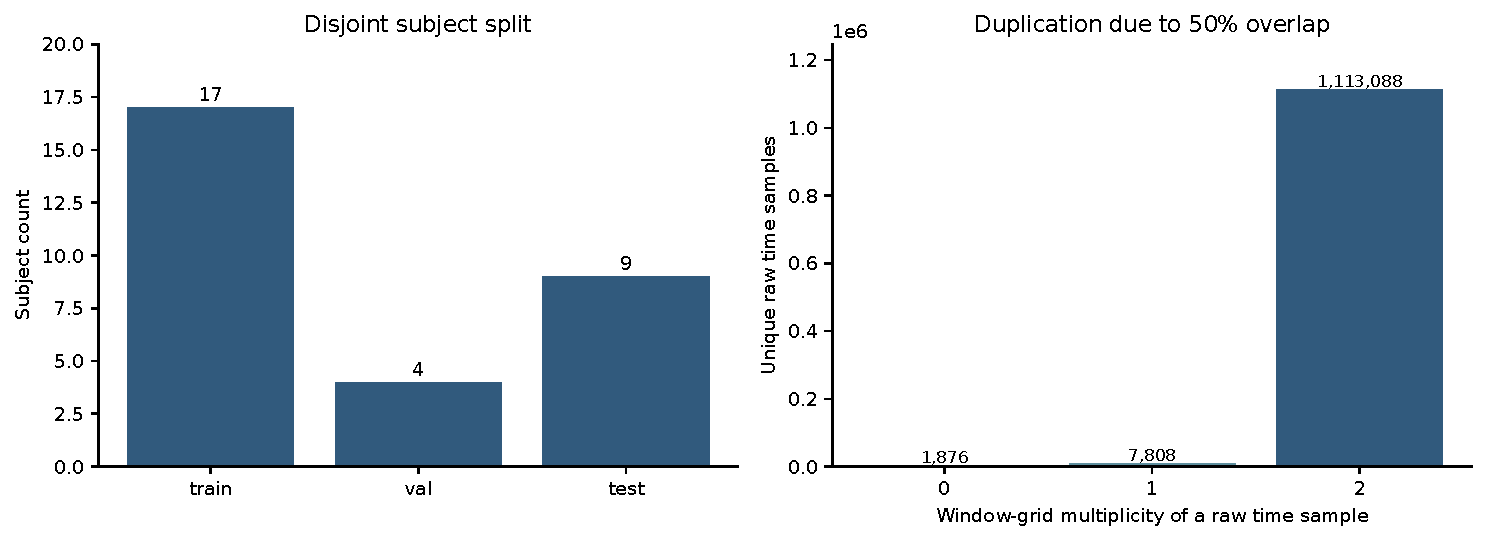
\includegraphics[width=\linewidth]{qa/data_cnn/data_split_multiplicity.pdf}
\caption{Disjoint subject partition and sample multiplicity histogram. Each raw time sample is counted exactly once in the multiplicity distribution ($m=0, 1, 2$).}
\end{figure}

\subsection{Aligned Overlap vs. Positional Difference}\label{sec:overlap_vs_delta}
A foundational property of ECDR is understanding the exact relationship between consecutive streaming queries.

\begin{definition}[Aligned Overlap Equality]
For any two chronologically adjacent windows $X_{e,k}$ and $X_{e,k+1}$ within the same recording session, the 50\% overlap ensures that the second half of window $k$ corresponds to the exact same physical time samples as the first half of window $k+1$:
\begin{equation}\label{eq:aligned_overlap}
X_{e,k}[c, 64 + i] = X_{e,k+1}[c, i] = r_e[kS + 64 + i, c], \quad \forall c \in \{1,\ldots,6\}, \; i \in \{0,\ldots,63\}.
\end{equation}
This is an \textbf{exact mathematical identity} representing identical raw memory locations placed at shifted tensor indices.
\end{definition}

\begin{definition}[Positional Delta Vector]
In contrast, the \textbf{positional delta} between adjacent windows compares sensory coordinates at identical tensor indices $i \in \{0, \ldots, 127\}$:
\begin{equation}\label{eq:positional_delta}
\Delta_{e,k}[c, i] \coloneqq X_{e,k+1}[c, i] - X_{e,k}[c, i] = r_e[kS + S + i, c] - r_e[kS + i, c].
\end{equation}
This vector measures the physical change of the signal across an elapsed duration of $S/50 = 1.28$~seconds.
\end{definition}

\begin{remark}[The Ramp Counterexample: Why Overlap Does Not Imply Small Delta]
The exact equality in \eqref{eq:aligned_overlap} does not imply that $\|\Delta_{e,k}\|_2$ or $\|\Delta_{e,k}\|_\infty$ is small. Consider a single-channel linear ramp signal $r[n] = n$. With $W=128, S=64$, window $k=0$ is $X_0 = [0, 1, \ldots, 127]$ and window $k=1$ is $X_1 = [64, 65, \ldots, 191]$. The aligned overlap is exact: $X_0[64:128] = X_1[0:64] = [64, 65, \ldots, 127]$. However, the positional delta is constant across all 128 coordinates:
\begin{equation*}
\Delta_0[i] = X_1[i] - X_0[i] = (64 + i) - i = 64, \quad \forall i \in \{0, \ldots, 127\}.
\end{equation*}
The $L_2$ norm of this delta is $\|\Delta_0\|_2 = \sqrt{128 \times 64^2} \approx 724.08$, and its $L_\infty$ norm is $64$. Although this linear ramp is an idealized pedagogical counterexample, it proves conclusively that 50\% overlap cannot mathematically guarantee small coordinate-wise perturbation bounds.
\end{remark}

Across the 61 sessions, the number of chronologically adjacent pairs is:
\begin{equation}
\sum_{e=1}^{61} (N_e - 1) = \sum_{e=1}^{61} N_e - 61 = 17,453 - 61 = 17,392\text{ adjacent pairs}.
\end{equation}
The total number of pairs is 17,392 (not $17,453 - 1 = 17,452$) because session boundaries cannot be paired. Each adjacent pair shares $6 \times 64 = 384$ coordinates, yielding $17,392 \times 384 = 6,678,528$ overlapping coordinates. Our audit verified every single coordinate: zero mismatches exist.

\section{Annotation and Labeling Policies: Defining Working Datasets}

\subsection{Inherited Annotation Conventions and Open Questions}
Each row in the raw annotation file \code{labels.txt} is a 5-tuple $(e, u, a, b_0, b_1)$ specifying recording session $e$, subject $u$, activity class $a \in \{1, \ldots, 12\}$, start index $b_0$, and end index $b_1$. The local pipeline interprets this interval under Python inclusive slice semantics: \code{labels[b_0 : b_1 + 1]}, spanning $b_1 - b_0 + 1$ samples. In contrast, sliding windows are sliced with 0-based exclusive upper bounds.

The dataset documentation is ambiguous regarding whether original raw indices were 0-based or 1-based. To ensure strict numerical reproducibility, this audit adheres to the inherited indexing convention of the existing codebase. Replicating existing numbers does not prove that this convention matches the original experimental intent; the exact indexing provenance must be formally resolved before freezing future production pipelines.

Under this convention, exactly 815,614 raw samples (72.64\%) possess activity annotations, while 307,158 samples (27.36\%) remain unannotated. Annotation coverage varies substantially across sessions, ranging from 39.21\% (exp12, user06) to 80.26\% (exp56, user28). Unannotated segments must not be naively imputed as stationary resting, sensor noise, or an unrecorded 13th activity.

\subsection{Formal Definitions of the Four Window Policies}
Let $n_a(X) \coloneqq \sum_{i=0}^{W-1} \mathbf{1}\{\text{label}(kS + i) = a\}$ denote the number of samples in window $X$ assigned activity ID $a \in \{1, \ldots, 12\}$.

\begin{definition}[Dominant Label Proportion]
The dominant activity proportion of window $X$ is defined as:
\begin{equation}
p_{\max}(X) \coloneqq \max_{a \in \{1, \ldots, 12\}} \frac{n_a(X)}{W}.
\end{equation}
The denominator is strictly the full window length ($W = 128$), including unannotated samples.
\end{definition}

The existing pipeline partitions all 17,453 windows into four mutually exclusive policies:
\begin{enumerate}
\item \textbf{Pure Window:} All 128 samples belong to the exact same positive activity class:
\begin{equation}
\exists a \in \{1, \ldots, 12\} \text{ such that } n_a(X) = 128 \iff p_{\max}(X) = 1.0.
\end{equation}
\item \textbf{Majority Window:} The window is not pure, but its dominant positive activity covers at least 60\% of the window:
\begin{equation}
p_{\max}(X) \ge 0.6 \iff n_{\text{majority}}(X) \ge \lceil 0.6 \times 128 \rceil = 77\text{ samples}.
\end{equation}
\item \textbf{Ambiguous Window:} The window contains at least one positive activity label, but the dominant class covers less than 60\% of the window ($0 < p_{\max}(X) < 0.6$, i.e., $n_{\text{majority}}(X) \le 76$).
\item \textbf{Unlabeled Window:} The window contains zero positive activity labels ($n_a(X) = 0$ for all $a \in \{1, \ldots, 12\}$, so $p_{\max}(X) = 0$; assigned metadata label ID 0).
\end{enumerate}

\begin{table}[htbp]\centering\small
\begin{tabularx}{\linewidth}{@{}P{2.4cm}Yrr@{}}\toprule
Window Policy & Formal Pipeline Condition & Window Count & Stream Proportion\\\midrule
\textbf{Pure} & Exactly 128 samples share one activity $a \in \{1,\ldots,12\}$. & 10,361 & 59.3652\%\\
\textbf{Majority} & Not pure; $\max_a n_a(X) \ge 77$ samples ($p_{\max} \ge 0.6$). & 1,917 & 10.9838\%\\
\textbf{Ambiguous} & Has positive labels; $\max_a n_a(X) \le 76$ samples ($p_{\max} < 0.6$). & 1,588 & 9.0987\%\\
\textbf{Unlabeled} & Zero positive labels ($n_a(X) = 0$ for all $a \ge 1$; majority ID is 0). & 3,587 & 20.5523\%\\\bottomrule
\end{tabularx}
\caption{Comprehensive census of window labeling policies across all 17,453 windows.}
\end{table}

\begin{remark}[Clarification on Policy Thresholding]
Consider a window containing 60 samples labeled class 4 (\code{SITTING}) and 68 unannotated samples. Because the denominator is 128, the proportion is $60/128 = 46.875\% < 60\%$. Therefore, this window is categorized as \textbf{ambiguous}, even though 100\% of its labeled samples belong to class 4. Furthermore, a window consisting of 128 samples of a postural transition (e.g., class 8: \code{SIT_TO_STAND}) is a \textbf{pure window}. ``Postural transition'' refers to the physical nature of the activity class, whereas ``ambiguous'' or ``mixed'' refers to label heterogeneity within the sliding window.
\end{remark}

Exactly 1,273 windows are flagged with \code{crosses_boundary = True} (7.2939\% of all windows). This metadata flag indicates that the window overlaps an annotation boundary; it is not synonymous with ambiguous. A window crossing a boundary can still achieve majority status if one class covers $\ge 77$ samples.

\begin{figure}[htbp]\centering
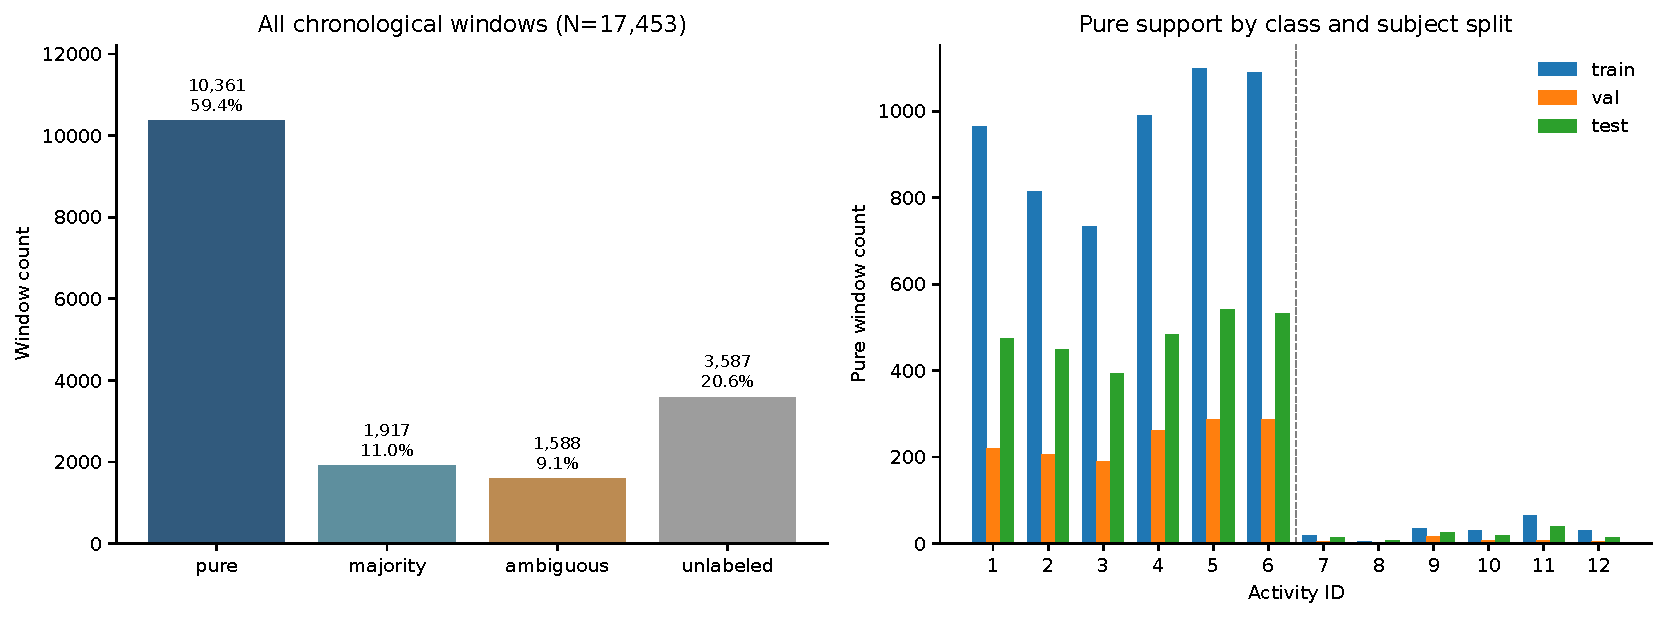
\includegraphics[width=\linewidth]{qa/data_cnn/data_policy_support.pdf}
\caption{Distribution of window policies across the full stream (left) and pure class support across subject splits (right). The vertical separator between ID 6 and ID 7 demarcates basic activities from postural transitions.}
\end{figure}

\section{Twelve Classes, Span Lengths, and Grid-Induced Bias}

\subsection{Actual Support After Window Slicing}
Table~\ref{tab:pure_class_support} presents the exact distribution of pure windows across all 12 classes and subject splits.

\begin{table}[htbp]\centering\small
\begin{tabular}{rllrrrr}\toprule
ID & Activity Name & Type & Train & Val & Test & Total\\\midrule
1 & \code{WALKING} & Basic activity & 965 & 221 & 474 & 1,660\\
2 & \code{WALKING_UPSTAIRS} & Basic activity & 814 & 205 & 449 & 1,468\\
3 & \code{WALKING_DOWNSTAIRS} & Basic activity & 734 & 189 & 394 & 1,317\\
4 & \code{SITTING} & Basic activity & 991 & 261 & 484 & 1,736\\
5 & \code{STANDING} & Basic activity & 1,099 & 286 & 541 & 1,926\\
6 & \code{LAYING} & Basic activity & 1,090 & 288 & 532 & 1,910\\
7 & \code{STAND_TO_SIT} & Postural transition & 19 & 5 & 15 & 39\\
8 & \code{SIT_TO_STAND} & Postural transition & 5 & 1 & 6 & 12\\
9 & \code{SIT_TO_LIE} & Postural transition & 36 & 16 & 25 & 77\\
10 & \code{LIE_TO_SIT} & Postural transition & 30 & 6 & 18 & 54\\
11 & \code{STAND_TO_LIE} & Postural transition & 65 & 7 & 40 & 112\\
12 & \code{LIE_TO_STAND} & Postural transition & 30 & 5 & 15 & 50\\\midrule
\multicolumn{3}{l}{Basic activities subtotal (Classes 1--6)} & 5,693 & 1,450 & 2,874 & 10,017\\
\multicolumn{3}{l}{Postural transitions subtotal (Classes 7--12)} & 185 & 40 & 119 & 344\\\midrule
\multicolumn{3}{l}{Full 12-class pure total} & 5,878 & 1,490 & 2,993 & 10,361\\\bottomrule
\end{tabular}
\caption{Pure window support across classes and splits under inherited conventions.}\label{tab:pure_class_support}
\end{table}

The basic activities (Classes 1--6) constitute 10,017 pure windows (96.68\% of all pure windows). The six postural transitions constitute only 344 pure windows (3.32\%). Filtering the problem down to 6 classes (as done in older repository checkpoints) discards the 344 transition windows and fundamentally changes the classification problem and evaluation denominator. If future ECDR research targets the full 12-class schema, all model heads, margin verifiers, and evaluation protocols must report performance on the 12-class population.

\subsection{Why Pure Support Collapses for Postural Transitions}
Table~\ref{tab:span_durations} summarizes the physical duration of continuous annotation spans.

\begin{table}[htbp]\centering\small
\begin{tabular}{rlrrrrr}\toprule
ID & Activity Name & Spans & Min (s) & Median (s) & Max (s) & Spans $<128$ samples\\\midrule
1 & \code{WALKING} & 127 & 2.82 & 19.36 & 28.22 & 0\\
2 & \code{WALKING_UPSTAIRS} & 183 & 4.44 & 12.68 & 17.90 & 0\\
3 & \code{WALKING_DOWNSTAIRS} & 186 & 4.32 & 11.77 & 17.60 & 0\\
4 & \code{SITTING} & 120 & 12.46 & 20.83 & 32.44 & 0\\
5 & \code{STANDING} & 120 & 15.20 & 22.57 & 40.64 & 0\\
6 & \code{LAYING} & 120 & 15.56 & 22.11 & 33.90 & 0\\
7 & \code{STAND_TO_SIT} & 60 & 1.80 & 3.33 & 6.14 & 7\\
8 & \code{SIT_TO_STAND} & 62 & 1.48 & 2.59 & 3.66 & 29\\
9 & \code{SIT_TO_LIE} & 60 & 2.72 & 4.04 & 6.52 & 0\\
10 & \code{LIE_TO_SIT} & 60 & 2.28 & 3.58 & 5.60 & 2\\
11 & \code{STAND_TO_LIE} & 58 & 2.78 & 4.73 & 9.88 & 0\\
12 & \code{LIE_TO_STAND} & 58 & 2.36 & 3.62 & 6.46 & 2\\\bottomrule
\end{tabular}
\caption{Duration statistics of continuous annotation spans by activity class.}\label{tab:span_durations}
\end{table}

While basic activity spans exhibit median durations of 11.77--22.57~seconds, postural transitions have medians of only 2.59--4.73~seconds. This physical brevity approaches the 2.56-second window duration ($W=128$). Although all 358 transition spans collectively contain 67,208 raw samples, the standard windowing procedure discards most of them from the pure subset.

\begin{proposition}[Pure Window Count Within an Annotation Span]\label{prop:pure_span_count}
Let $[a, b]$ denote an inclusive annotation span ($a, b \in \mathbb{N}_0, b \ge a$) representing a single activity within a recording session. Let sliding windows of length $W$ start at indices $kS$ for $k \in \mathbb{N}_0$. The number of pure windows falling strictly within $[a, b]$ is:
\begin{equation}\label{eq:pure_span}
N_{[a, b]} = \max\left\{0, \; \left\lfloor \frac{b - W + 1}{S} \right\rfloor - \left\lceil \frac{a}{S} \right\rceil + 1 \right\}.
\end{equation}
\end{proposition}
\begin{proof}
Window $k$ is contained in $[a, b]$ if and only if its start index satisfies $kS \ge a$ and its end index satisfies $kS + W - 1 \le b$. The first inequality requires $k \ge a/S$. Since $k$ is an integer, this imposes the lower bound $k \ge \lceil a/S \rceil$. The second inequality requires $kS \le b - W + 1$, imposing the upper bound $k \le \lfloor (b - W + 1)/S \rfloor$. The number of integers in the interval $[k_{\min}, k_{\max}]$ is $\max\{0, k_{\max} - k_{\min} + 1\}$, proving \eqref{eq:pure_span}.
\end{proof}

\begin{remark}[The Stride-Grid Phase Penalty]
The condition $b - a + 1 \ge 128$ is a necessary condition for $N_{[a,b]} \ge 1$, but it is \textbf{not sufficient}. For example, consider a span spanning indices $[1, 128]$, which has length exactly $128 - 1 + 1 = 128$ samples. By Proposition~\ref{prop:pure_span_count} with $W=128, S=64$:
\begin{equation*}
k_{\min} = \lceil 1/64 \rceil = 1, \qquad k_{\max} = \lfloor (128 - 128 + 1)/64 \rfloor = \lfloor 1/64 \rfloor = 0.
\end{equation*}
Since $k_{\max} < k_{\min}$, $N_{[1, 128]} = 0$. Window $k=0$ begins at 0 and ends at 127 (excluding sample 128), while window $k=1$ begins at 64 and ends at 191 (including samples beyond the span). Thus, despite spanning 128 samples, the span produces \textbf{zero pure windows}.
Conversely, span $[64, 191]$ also has length 128, but its phase aligns perfectly: $k_{\min} = \lceil 64/64 \rceil = 1, k_{\max} = \lfloor (191 - 128 + 1)/64 \rfloor = 1$, yielding $N_{[64, 191]} = 1$.
\end{remark}

Across the 1,214 annotation spans in the dataset:
\begin{itemize}
\item Exactly 40 spans are strictly shorter than 128 samples (all are postural transitions).
\item Exactly 91 spans have length $\ge 128$ samples but yield zero pure windows due to stride-grid phase misalignment (1 basic activity span, 90 transition spans).
\item Exactly 1,083 spans contain at least one aligned pure window (855 basic, 228 transition).
\end{itemize}
Summing \eqref{eq:pure_span} across all 1,214 spans yields exactly 10,361 pure windows, matching the empirical support identically. For \code{SIT_TO_STAND} (Class 8), out of 62 spans, 29 are shorter than 128 samples, 21 are long enough but misaligned with the stride grid, leaving only 12 spans that produce pure windows (yielding a dataset-wide total of 12 windows).

This combinatorial mechanism proves that the scarcity of transition windows is an artifact of the discretization grid. Altering the stride, employing variable window lengths, or training on soft multi-label distributions represent distinct methodological interventions that would require establishing a new evaluation protocol.

\section{Splits, Statistical Dependence, and Evaluation Units}

\subsection{Subject-Disjoint Splits and Slicing Metadata}
\begin{table}[htbp]\centering\small
\begin{tabular}{lrrrrrr}\toprule
Split & Subjects & Recordings & Raw Samples & All Windows & Pure K12 & Pure K6\\\midrule
Train & 17 & 34 & 641,745 & 9,978 & 5,878 & 5,693\\
Validation & 4 & 8 & 155,739 & 2,422 & 1,490 & 1,450\\
Test & 9 & 19 & 325,288 & 5,053 & 2,993 & 2,874\\\midrule
Total & 30 & 61 & 1,122,772 & 17,453 & 10,361 & 10,017\\\bottomrule
\end{tabular}
\caption{Subject-disjoint data split partitioning in the local workspace.}
\end{table}

The subject sets across splits are strictly mutually disjoint:
\begin{itemize}
\item \textbf{Train Subjects (17):} 1, 3, 5, 6, 7, 8, 11, 14, 15, 16, 17, 19, 21, 22, 23, 25, 26.
\item \textbf{Validation Subjects (4):} 27, 28, 29, 30.
\item \textbf{Test Subjects (9):} 2, 4, 9, 10, 12, 13, 18, 20, 24.
\end{itemize}

The number of adjacent window pairs by split is: Train 9,944; Validation 2,414; Test 5,034. These counts equal the number of windows minus the number of sessions in each split ($\sum_{e \in \text{split}} (N_e - 1)$). The pure test subset of 2,874 windows applies strictly to the filtered 6-class static/locomotion subset; it must never be used as the denominator for decision reuse across the full test stream (which contains 5,053 query windows and 5,034 adjacent pairs).

\subsection{Why 17,453 Windows Are Not Independent and Identically Distributed (i.i.d.)}
A fundamental statistical error is treating all 17,453 windows as independent observations:
\begin{enumerate}
\item \textbf{Direct Sample Overlap:} Adjacent windows share 50\% of their raw sensor coordinates ($6 \times 64 = 384$ shared numbers).
\item \textbf{Intra-Subject Correlation:} Multiple recordings from the same human participant share individual gait dynamics, body mass, phone placement angle, and movement style.
\end{enumerate}

For any sample mean $\bar{Z} = N^{-1} \sum_{i=1}^N Z_i$, the true sampling variance is:
\begin{equation}
\operatorname{Var}(\bar{Z}) = \frac{1}{N^2} \sum_{i=1}^N \sum_{j=1}^N \operatorname{Cov}(Z_i, Z_j) = \frac{\sigma^2}{N} + \frac{1}{N^2} \sum_{i \ne j} \operatorname{Cov}(Z_i, Z_j).
\end{equation}
Simplifying this to $\sigma^2 / N$ requires that all off-diagonal covariance terms vanish. Due to 50\% window overlap and subject clustering, off-diagonal covariances are strongly positive. Consequently, standard sample standard errors drastically underestimate true parameter uncertainty.

Furthermore, one cannot calculate an ``effective sample size'' $N_{\text{eff}}$ purely based on 50\% geometric overlap. Classifier decisions, non-linear activation boundaries, and activity duration exhibit complex, heterogeneous dependencies. Rigorous inferential evaluation requires block-bootstrapping or clustering at the subject level, acknowledging that the validation split contains only four subjects.

\subsection{The Role of Test Data in an Exploratory Audit}
The descriptive statistics and empirical distributions presented in this report examine all three splits to characterize the physical reality of the dataset. Therefore, these tables do not serve as a blind, held-out validation of an adaptive algorithm. If hyper-parameters, perturbation budgets, or network architectures are tuned based on whole-dataset distance percentiles, that choice must be documented, and formal confirmation must be conducted on an independent, unseen test stream.

\section{Channel Distributions, Scales, and Normalization Geometry}

\subsection{Raw Descriptive Statistics on Unique Samples}
Table~\ref{tab:channel_stats} reports the physical distributions computed across all 1,122,772 unique raw time samples without overlap duplication.

\begin{table}[htbp]\centering\small
\begin{tabular}{llrrrrrrr}\toprule
Channel & Unit & Mean & Std ($\sigma$) & Min & p01 & p50 (Median) & p99 & Max\\\midrule
\code{acc_x} & $g$ & 0.81933 & 0.39612 & $-1.97639$ & $-0.17083$ & 0.96250 & 1.65694 & 2.00417\\
\code{acc_y} & $g$ & $-0.00789$ & 0.37401 & $-2.00972$ & $-0.72361$ & $-0.10139$ & 0.97639 & 1.71667\\
\code{acc_z} & $g$ & 0.08220 & 0.36043 & $-1.83750$ & $-0.68056$ & 0.02917 & 0.99306 & 1.97917\\
\code{gyro_x} & $\mathrm{rad/s}$ & 0.02085 & 0.58069 & $-9.88441$ & $-1.91995$ & 0.00764 & 1.90018 & 10.00353\\
\code{gyro_y} & $\mathrm{rad/s}$ & $-0.00832$ & 0.45466 & $-10.00842$ & $-1.27182$ & 0.00031 & 1.34879 & 9.98887\\
\code{gyro_z} & $\mathrm{rad/s}$ & $-0.01065$ & 0.34865 & $-10.00842$ & $-1.04489$ & $-0.00031$ & 0.94440 & 10.00353\\\bottomrule
\end{tabular}
\caption{Raw channel distributions across 1,122,772 unique time samples (population std, ddof=0).}\label{tab:channel_stats}
\end{table}

The mean of \code{acc_x} is $+0.81933\,g$, far from zero. This reflects the orientation of the waist-mounted phone under gravitational acceleration. Accelerometer channels are bounded within $[-2.01, +2.00]\,g$, and gyroscope channels within $[-10.01, +10.00]\,\mathrm{rad/s}$. These values describe the physical data; they do not represent universal constants of human motion.

\begin{figure}[htbp]\centering
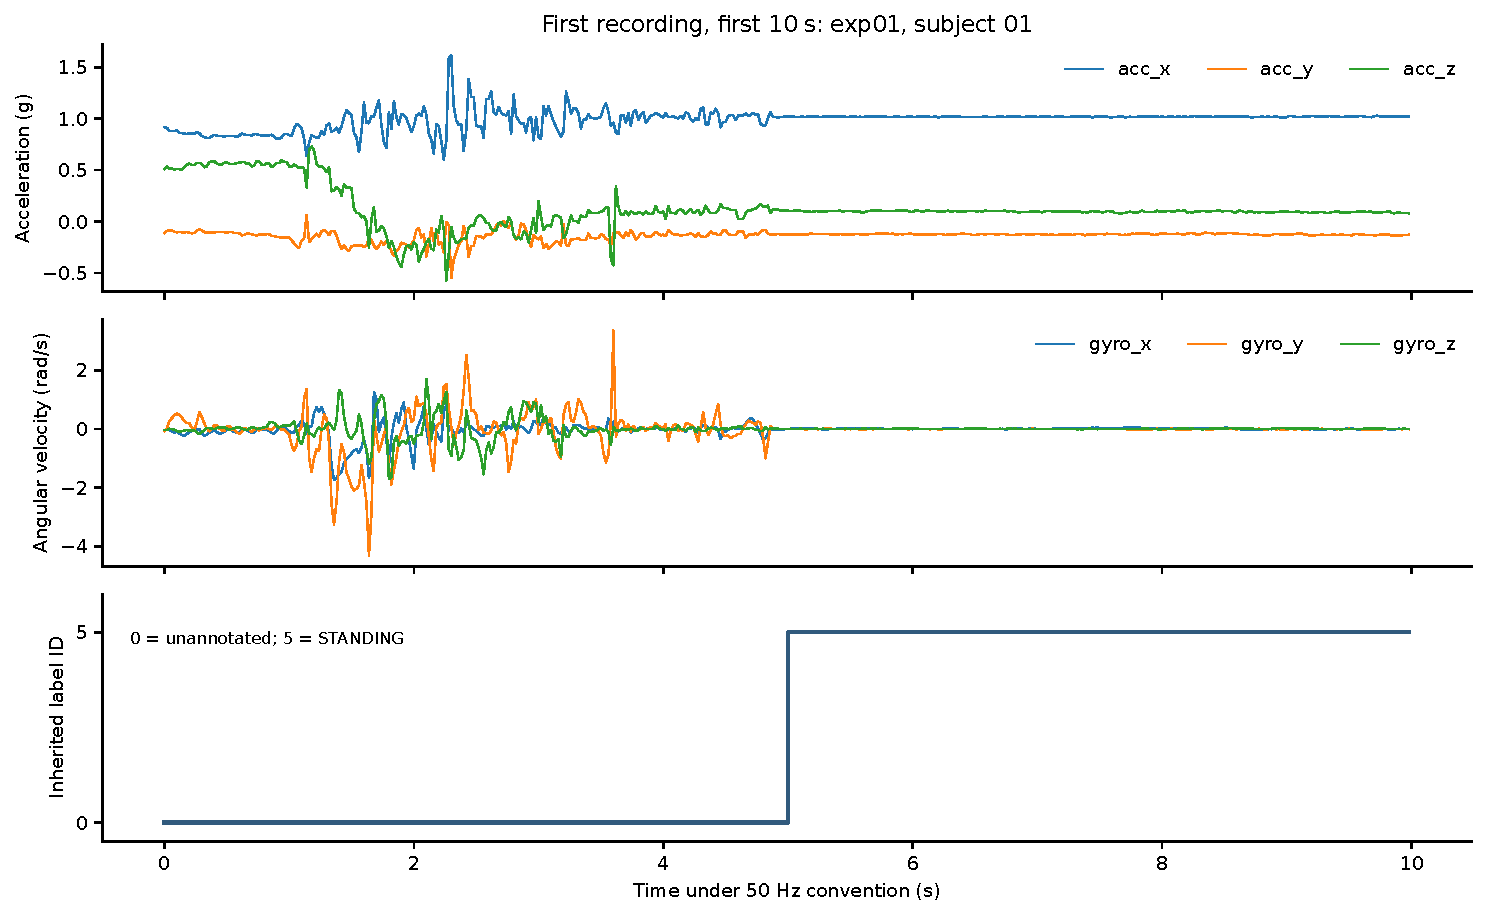
\includegraphics[width=0.98\linewidth]{qa/data_cnn/data_raw_first_recording.pdf}
\caption{First 10 seconds of raw session \code{exp01} (subject 01). Sourced deterministically to illustrate sensor reading ranges and initial unannotated/standing states; not cherry-picked for classification performance.}
\end{figure}

\subsection{Standardization Parameters in the Local Audit}
To enable distance calculations across heterogeneous physical dimensions ($g$ vs. $\mathrm{rad/s}$), the local audit applies channel-wise standardization using parameters fitted exclusively on the 5,693 pure 6-class training windows:
\begin{equation}
Z[c, i] = \frac{X[c, i] - \mu_c}{\sigma_c}, \quad \mu_c = \frac{1}{128 N_{\text{tr}}} \sum_{w \in \text{tr}} \sum_{i=0}^{127} X_w[c, i],
\end{equation}
with standard deviations clipped to a minimum of $10^{-6}$. The fixed numerical parameters are:
\begin{center}\small
\begin{tabular}{@{}lrr@{}}\toprule
Channel & Fitted Mean ($\mu_c$) & Fitted Std ($\sigma_c$)\\\midrule
\code{acc_x} & 0.804849 & 0.413195\\
\code{acc_y} & 0.030074 & 0.402293\\
\code{acc_z} & 0.080927 & 0.356522\\
\code{gyro_x} & 0.004974 & 0.417901\\
\code{gyro_y} & $-0.002906$ & 0.406792\\
\code{gyro_z} & $-0.007806$ & 0.261610\\\bottomrule
\end{tabular}
\end{center}

Because these parameters were fitted across overlapping training windows, raw samples were implicitly weighted by their multiplicity $m_e[n]$. Furthermore, postural transitions were excluded from the fit. If future work trains a 12-class classifier, standardization parameters must be fitted on an appropriate population and frozen prior to evaluation.

\subsection{Geometric Distortion Under Normalization}
Standardization fundamentally alters the geometry of perturbation neighborhoods:
\begin{definition}[Affine Metric Distortion]
Let $D \coloneqq \operatorname{diag}(\sigma_1, \ldots, \sigma_6) \otimes I_{128}$ denote the $768 \times 768$ diagonal scaling matrix. The normalized perturbation vector $\Delta z$ and its Euclidean norm satisfy:
\begin{equation}
\Delta z = D^{-1} \Delta x, \qquad \|\Delta z\|_2^2 = \sum_{c=1}^6 \sum_{i=0}^{127} \frac{\Delta x[c, i]^2}{\sigma_c^2}.
\end{equation}
\end{definition}

In raw sensor space, computing a naive Euclidean distance adds $g^2$ directly to $(\mathrm{rad/s})^2$---an operation lacking physical dimensional meaning. Normalized coordinates resolve this unit mismatch, but the metric remains dependent on the normalization population.

Crucially, an isotropic $L_2$ ball in normalized space ($\|\Delta z\|_2 \le \epsilon$) corresponds to a multi-axial hyper-ellipsoid in raw sensor space:
\begin{equation}
\mathcal{E} \coloneqq \left\{ \Delta x \in \R^{6 \times 128} : \sum_{c=1}^6 \frac{1}{\sigma_c^2} \sum_{i=0}^{127} \Delta x[c, i]^2 \le \epsilon^2 \right\}.
\end{equation}
Similarly, an $L_\infty$ box bound $|\Delta x[c, i]| \le b_c$ corresponds to the normalized box $|\Delta z[c, i]| \le b_c / \sigma_c$. Coordinate systems must remain strictly identical across domain construction, membership testing, and classifier certification $F = f_\theta \circ N$. If per-instance z-score normalization were applied dynamically to each window, $N$ would become non-linear, invalidating all affine certificates.

\section{Temporal Continuity: Four Types of Autocorrelation}

\subsection{Distinguishing Correlation Metrics}
The Pearson correlation between vectors $a, b \in \R^m$ is:
\begin{equation}
\operatorname{corr}(a, b) = \frac{\sum_{i=1}^m (a_i - \bar{a})(b_i - \bar{b})}{\sqrt{\sum_{i=1}^m (a_i - \bar{a})^2 \sum_{i=1}^m (b_i - \bar{b})^2}}.
\end{equation}
To prevent conflating distinct physical questions, we compute four separate autocorrelation measures:
\begin{enumerate}
\item \textbf{Raw Lag-1 Autocorrelation:} The correlation between $r_e[0 : T_e - 1, c]$ and $r_e[1 : T_e, c]$, reflecting temporal dependence across an interval of 20~ms.
\item \textbf{Raw Lag-64 Autocorrelation:} The correlation between $r_e[0 : T_e - 64, c]$ and $r_e[64 : T_e, c]$, reflecting temporal dependence across the query stride of 1.28~s.
\item \textbf{Window Positional Correlation:} The correlation between the 128-dimensional vectors of window $k$ and window $k+1$ at identical tensor indices (\eqref{eq:positional_delta}).
\item \textbf{Window Channel-Mean Correlation:} Letting $g_k \coloneqq \frac{1}{128} \sum_{i=0}^{127} X_{e,k}[c, i]$, the correlation between the sequence $(g_0, \ldots, g_{N_e-2})$ and $(g_1, \ldots, g_{N_e-1})$ across consecutive windows.
\end{enumerate}

Each metric is evaluated within each recording session and averaged across all 61 sessions:

\begin{table}[htbp]\centering\small
\begin{tabular}{lrrrr}\toprule
Channel & Raw Lag-1 (20 ms) & Raw Lag-64 (1.28 s) & Window Positional & Window Channel-Mean\\\midrule
\code{acc_x} & 0.9716 & 0.7209 & 0.0119 & 0.9661\\
\code{acc_y} & 0.9778 & 0.8240 & 0.0224 & 0.9717\\
\code{acc_z} & 0.9773 & 0.7769 & 0.0485 & 0.9360\\
\code{gyro_x} & 0.9550 & 0.1484 & $-0.0307$ & 0.6614\\
\code{gyro_y} & 0.8297 & 0.0606 & $-0.0137$ & 0.5596\\
\code{gyro_z} & 0.9183 & 0.0960 & $-0.0095$ & 0.6134\\\bottomrule
\end{tabular}
\caption{Empirical temporal correlation across channels under four distinct formulations.}
\end{table}

\subsection{Physical Interpretation and an Artifact Discovery}
The empirical results reveal crucial structural properties:
\begin{itemize}
\item Raw Lag-1 is exceedingly high ($0.83 - 0.98$), consistent with smooth physical sensor motion over 20~ms.
\item At Lag-64 (1.28~s), gyroscope autocorrelation drops sharply to $0.06 - 0.15$, whereas accelerometer autocorrelation remains robust ($0.72 - 0.82$). High 20~ms correlation cannot be naively extrapolated to the 1.28~s query stride.
\item Window positional correlation is near zero ($-0.03$ to $+0.05$). This does not contradict exact overlap: positional correlation compares samples separated by 1.28~s (\eqref{eq:positional_delta}).
\item Window channel-mean correlation is substantial ($0.56 - 0.97$), demonstrating that spatial orientation averages remain stable over time even when high-frequency waveform shapes change.
\end{itemize}

\begin{remark}[Identification of a Codebase Pipeline Bug]
Our audit discovered that an older audit script in the workspace (\code{scripts/06b_corr_semantics.py}) generated a pseudo-raw time series by applying \code{ravel()} to the 3D tensor of overlapping windows. Because windows overlap by 50\%, flattening the tensor repeats samples and introduces severe artificial discontinuities at window boundaries. Consequently, the correlation numbers stored in \code{data/corr_semantics.json} are mathematically compromised. The clean numbers in Table~\ref{tab:channel_stats} were recomputed directly on uninterrupted raw text files.
\end{remark}

\section{Inter-Window Distances: Stratification vs. Pooled Metrics}

\subsection{Partitioning Adjacent Window Pairs}
All 17,392 adjacent window pairs are partitioned into three mutually exclusive categories:
\begin{enumerate}
\item \textbf{Same-Activity Pure Pairs (9,278 pairs):} Both windows are pure and share the exact same activity label ($a_k = a_{k+1}$).
\item \textbf{Majority-Label Change Pairs (1,651 pairs):} The dominant majority label changes between window $k$ and window $k+1$.
\item \textbf{Equal-Majority Non-Pure Pairs (6,463 pairs):} Both windows share the same majority label, but at least one window is non-pure or unlabeled.
\end{enumerate}

Let $d_2 \coloneqq \|\operatorname{vec}(Z_{k+1} - Z_k)\|_2$ and $d_\infty \coloneqq \max_{c, i} |Z_{k+1}[c, i] - Z_k[c, i]|$. In $\R^{768}$:
\begin{equation}
d_\infty \le d_2 \le \sqrt{768} \, d_\infty \approx 27.7128 \, d_\infty.
\end{equation}
These bounds relate the two norms for an individual vector; they do not allow percentiles of one norm to be translated into exact percentiles of the other.

\begin{table}[htbp]\centering\small
\begin{tabular}{llrrr}\toprule
Coordinate System & Pair Subset and Norm & p50 (Median) & p90 & p99\\\midrule
Raw (mixed units) & Same-pure / $L_2$ & 1.84282 & 17.35410 & 24.18713\\
Raw (mixed units) & Majority-change / $L_2$ & 13.26583 & 22.97948 & 29.56845\\
Normalized & Same-pure / $L_2$ & 4.93575 & 46.41709 & 65.26317\\
Normalized & Majority-change / $L_2$ & 36.56520 & 59.33480 & 77.60553\\
Normalized & Same-pure / $L_\infty$ & 0.98734 & 7.06383 & 12.31258\\
Normalized & Majority-change / $L_\infty$ & 5.81409 & 9.47326 & 15.07550\\\bottomrule
\end{tabular}
\caption{Empirical distance quantiles across adjacent window pairs in the snapshot.}
\end{table}

\begin{figure}[htbp]\centering
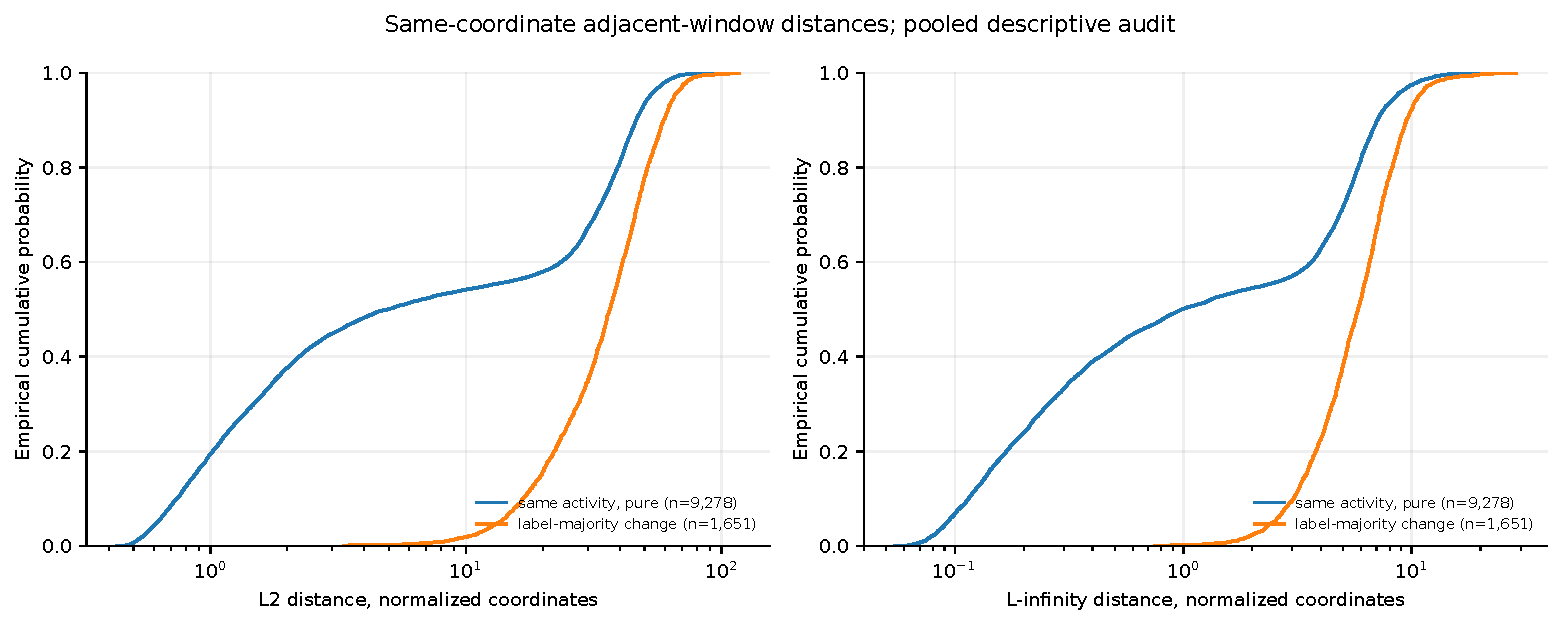
\includegraphics[width=\linewidth]{qa/data_cnn/data_normalized_distances.pdf}
\caption{Empirical Cumulative Distribution Functions (ECDF) of normalized $L_2$ and $L_\infty$ distances on a logarithmic scale. The two distributions overlap substantially; no classification decision boundary is evaluated in this figure.}
\end{figure}

Although the median distance between same-pure pairs is lower than that of majority-change pairs, their distributions overlap heavily. One cannot pick a quantile threshold and assert that all pairs below it share the same prediction. Ground-truth activity metadata is not identical to model behavior: a neural network may misclassify an input or exhibit sensitivity to phase shifts even when the ground-truth activity remains unchanged.

\subsection{Per-Class Breakdown: Why Pooled Medians Conceal Structure}
Table~\ref{tab:class_distances} stratifies same-pure adjacent pairs by activity class.

\begin{table}[htbp]\centering\small
\begin{tabular}{rlrrr}\toprule
Activity ID & Activity Name & Same-Pure Pairs & Median Normalized $L_2$ & p90 Normalized $L_2$\\\midrule
1 & \code{WALKING} & 1,534 & 36.43503 & 49.93195\\
2 & \code{WALKING_UPSTAIRS} & 1,285 & 32.85961 & 47.99001\\
3 & \code{WALKING_DOWNSTAIRS} & 1,131 & 44.86683 & 60.33992\\
4 & \code{SITTING} & 1,616 & 1.08972 & 3.62727\\
5 & \code{STANDING} & 1,806 & 1.75657 & 7.56076\\
6 & \code{LAYING} & 1,790 & 1.35659 & 3.95880\\
7 & \code{STAND_TO_SIT} & 8 & 45.95473 & 57.19978\\
8 & \code{SIT_TO_STAND} & 0 & Undefined & Undefined\\
9 & \code{SIT_TO_LIE} & 27 & 45.08910 & 53.99518\\
10 & \code{LIE_TO_SIT} & 13 & 41.32653 & 49.87594\\
11 & \code{STAND_TO_LIE} & 57 & 39.92019 & 51.32326\\
12 & \code{LIE_TO_STAND} & 11 & 39.97517 & 49.35115\\\bottomrule
\end{tabular}
\caption{Adjacent same-pure normalized $L_2$ distance quantiles by activity class.}\label{tab:class_distances}
\end{table}

The data reveals an extreme structural bifurcation:
\begin{itemize}
\item \textbf{Static Postures (Classes 4--6):} Display small median distances ($1.09 - 1.76$). Variations are primarily driven by sensor noise and respiration.
\item \textbf{Locomotion Activities (Classes 1--3):} Display large median distances ($32.86 - 44.87$), comparable to transitions. Gait cycles introduce large positional shifts over a 1.28~s stride.
\item \textbf{Postural Transitions (Classes 7--12):} Exhibit high median distances ($39.92 - 45.95$). Class 8 (\code{SIT_TO_STAND}) contains zero adjacent pure pairs.
\end{itemize}

A single global distance threshold would either encompass enormous noise for static postures or completely exclude locomotion from reuse. In production streaming, runtime event detectors cannot access ground-truth activity labels to choose thresholds; any activity-conditional threshold must rely strictly on causal, pre-classification signals.

\section{From Data Foundations to ECDR Perturbation Domains}

\subsection{The Mathematical Framework of Sound Decision Reuse}
Let $N: \R^{6 \times 128} \to \R^{6 \times 128}$ denote fixed normalization, $f_\theta: \R^{6 \times 128} \to \R^K$ denote the neural network producing raw logits, and $F \coloneqq f_\theta \circ N$.
Let $X^r$ denote an anchor window evaluated by the reference model, yielding top prediction $c = \arg\max_j F_j(X^r)$. Let $\mathcal{S}_e(X^r)$ denote an input perturbation domain centered around $X^r$.

\begin{definition}[Sound Decision Reuse Condition]
The reference decision $c$ is guaranteed to hold for query $X_t$ if:
\begin{equation}\label{eq:cert_condition}
X_t \in \mathcal{S}_e(X^r) \qquad \text{and} \qquad \underline{m}_{cj}\big(\mathcal{S}_e(X^r)\big) > 0, \quad \forall j \ne c,
\end{equation}
where $\underline{m}_{cj}(\mathcal{S}) \le \inf_{X \in \mathcal{S}} [F_c(X) - F_j(X)]$ is a mathematically sound lower bound on the logit margin over the entire continuous domain $\mathcal{S}$.
\end{definition}

Data audits establish whether empirical queries $X_t$ satisfy membership $X_t \in \mathcal{S}_e(X^r)$. The neural network and formal verifier determine whether the margin lower bound $\underline{m}_{cj}$ remains strictly positive. Empirical data density within $\mathcal{S}$ cannot substitute for a formal verification certificate.

\begin{table}[htbp]\centering\small
\begin{tabularx}{\linewidth}{@{}P{3.2cm}Y Y@{}}\toprule
Empirical Observation & Principled Domain Formulation & Required Formal and Empirical Proof\\\midrule
Exact overlap after 64-sample time shift & Shift-plus-tail domain or wave-domain decomposition. & Rigorous bound on tail coordinates; handling of boundary convolutions and margin certification.\\
Channel-dependent physical scale & Diagonal hyper-rectangular box domain in normalized space. & Correct coordinate matching during membership testing; tight class-pair margin bounds.\\
Class-dependent distance scales & Multi-template domains selected via streaming runtime cues. & Causal selector without label oracle; independent evaluation of selector latency and false positive costs.\\
Channel means more stable than waveforms & Structured domain combining low-rank projection with bounded residual. & Verification holds for all admissible residuals; residual bounds cannot rely on average reconstruction error.\\
Postural transitions have scarce support & Disaggregated reporting across basic classes, transitions, and mixed streams. & Reference model reliability verified on transitions; no artificial exclusion of challenging stream segments.\\\bottomrule
\end{tabularx}
\caption{Connecting empirical data properties to domain architectures and proof obligations.}
\end{table}

\subsection{Why Marginal Quantiles Do Not Guarantee Joint Set Membership}
Suppose an audit fits coordinate-wise bounds $b_i$ as the 90th percentile of $|\Delta z_i|$ across training pairs. This constructs a bounding box $\mathcal{B} = \prod_{i=1}^{768} [-b_i, b_i]$.

\begin{remark}[The Curse of High Dimensionality in Joint Membership]
The marginal probability $\mathbb{P}(|\Delta z_i| \le b_i) = 0.90$ for each coordinate $i \in \{1, \ldots, 768\}$ does \textbf{not} imply that $\mathbb{P}(\Delta z \in \mathcal{B}) \ge 0.90$. In the hypothetical pedagogical case of independent coordinates:
\begin{equation}
\mathbb{P}(\Delta z \in \mathcal{B}) = \prod_{i=1}^{768} \mathbb{P}(|\Delta z_i| \le b_i) = 0.90^{768} \approx 7.215 \times 10^{-36}.
\end{equation}
Although sensory coordinates exhibit strong local covariance, empirical joint membership is always substantially lower than marginal percentiles. Conversely, union bounds $\mathbb{P}(\exists i : |\Delta z_i| > b_i) \le \sum_i \mathbb{P}(|\Delta z_i| > b_i)$ exceed 1.0 when dimension is high, providing vacuous bounds.
\end{remark}

Even if empirical joint membership is measured directly on a dataset, high empirical coverage merely indicates that recorded data points frequently fall within the set. It does not prove that the classifier's margin remains positive over every continuous point in $\mathcal{S}$. An excessively large domain captures high empirical data but fails formal certification; an excessively small domain certifies easily but yields zero practical reuse coverage.

\subsection{Wave-Domain Parameterization: Retaining Structure Without Ignoring Residuals}
In normalized coordinates, a structured wave-domain models streaming queries as:
\begin{equation}
z_t = T_S z^r + V u + \rho, \qquad u \in \mathcal{U}, \quad \rho \in \mathcal{R},
\end{equation}
where $T_S$ represents temporal shift matching the 64-sample overlap with appropriate boundary handling; $V \in \R^{768 \times p}$ is an orthonormal basis capturing low-frequency motion modes (e.g., via Principal Component Analysis); $\mathcal{U} \subset \R^p$ is a compact parameter set; and $\rho \in \mathcal{R} \subset \R^{768}$ is a bounded residual.

\begin{remark}[Residual Obligations]
If $V$ is fitted via PCA, the explained variance ratio represents an \emph{average} squared reconstruction error over training data. It does \textbf{not} imply that $\rho = 0$ or that future streaming residuals are universally small. Sound certification requires establishing rigorous $L_\infty$ or $L_2$ bounds on the residual set $\mathcal{R}$.
\end{remark}

Consider an idealized harmonic motion $s[n] = A \sin(\omega n + \phi)$. The positional delta across stride $S$ is:
\begin{equation}
s[n+S] - s[n] = 2 A \sin\left(\frac{\omega S}{2}\right) \cos\left(\omega n + \phi + \frac{\omega S}{2}\right).
\end{equation}
When $\omega S / 2 \approx \pi / 2$, the positional delta reaches an amplitude of $2A$, despite the underlying motion being perfectly periodic and identical in shape. This explains why structured temporal domains that explicitly account for phase shifts are vastly superior to naive Euclidean balls.

\subsection{Single-Step Proximity Does Not Ensure Multi-Step Anchor Lifetime}
Adjacent window statistics characterize one-step transitions ($X_{t+1}$ given $X_t$). In contrast, reusing decision $c$ across an extended horizon requires maintaining membership relative to an older anchor: $X_{t} \in \mathcal{S}(X^r)$ for $t - r \ge 1$.

By the triangle inequality:
\begin{equation}
\|X_t - X^r\| \le \sum_{i=r}^{t-1} \|X_{i+1} - X_i\|.
\end{equation}
A sequence of individually small adjacent perturbations can accumulate into substantial drift, exiting the certified domain.

\begin{remark}[The Stale Certificate Hazard: No Recentering Without Re-Verification]
A system must never dynamically recenter its certificate to a newly accepted query $X_t$ without executing a full verifier pass. If an anchor certificate guarantees that decision $c$ holds on $\mathcal{S}(X^r)$, that guarantee applies strictly to points within $\mathcal{S}(X^r)$. Moving the center to $X_t$ creates a new domain $\mathcal{S}(X_t)$ containing unexplored regions outside $\mathcal{S}(X^r)$ where competitive logits may cross. Measuring anchor lifetime requires true sequential replay with explicit state lifecycle tracking.
\end{remark}

\section{Evaluation Protocols Demanded by Empirical Data}

\subsection{Categorizing Experimental Evaluation Metrics}
A complete empirical evaluation of ECDR must decouple four distinct evaluation criteria:
\begin{enumerate}
\item \textbf{Reference Classifier Accuracy:} The agreement between model predictions and ground-truth activity annotations on a defined population.
\item \textbf{Decision Reuse Agreement:} The probability that the reused decision matches the exact prediction the reference classifier would have made on the same query ($c_{\text{reuse}} = \arg\max_j F_j(X_t)$).
\item \textbf{Sound Certification Rate:} The proportion of queries where the mathematical implication in \eqref{eq:cert_condition} holds with guaranteed numerical soundness.
\item \textbf{Net Computational Savings:} The reduction in overall execution latency and energy after accounting for selector overhead, membership checking, and certificate construction.
\end{enumerate}

High accuracy on a filtered pure test subset does not establish safety on a continuous mixed stream. If a reference model misclassifies a true activity, an ECDR system that faithfully reproduces the reference model's prediction will also output an incorrect label. Therefore, reference accuracy, certified reuse coverage, and runtime savings must be reported simultaneously across well-defined denominators.

\begin{table}[htbp]\centering\small
\begin{tabularx}{\linewidth}{@{}P{3.2cm}Y Y@{}}\toprule
Metric & Transparent Evaluation Denominator & Status in This Audit Snapshot\\\midrule
Pure K12 Accuracy & 2,993 pure test windows under the existing split. & Baseline CNN K12 training not yet executed.\\
All-Stream Membership & 5,053 test queries, or 5,034 adjacent test pairs. & Pending selection of final domain geometry.\\
Per-Class Coverage & Queries stratified by activity ID, explicitly including transition classes with low support. & Empirical support mapped; formal certification pending.\\
Multi-Step Reuse Horizon & Sequential queries replayed chronologically within recording sessions. & Requires end-to-end verifier streaming replay.\\
Net Computational Gain & Total time including selector, membership, verifier, and reference fallback passes. & Latency benchmarks not performed in this data audit.\\\bottomrule
\end{tabularx}
\caption{Required experimental metrics and their corresponding denominators.}
\end{table}

\subsection{System Cost Model and Break-Even Conditions}
Let $T_e$ denote the execution latency of the runtime event selector; let $T_m$ denote the latency of the domain membership test; let $T_f$ denote the full inference latency of the reference neural network; let $T_b$ denote the computational cost of building a certificate when refreshing an anchor; let $r \in [0, 1]$ denote the certified reuse rate; and let $q \in [0, 1]$ denote the anchor refresh rate per query.

The expected inference latency per streaming query is:
\begin{equation}
\mathbb{E}[T_{\text{query}}] \approx T_e + T_m + (1 - r) T_f + q T_b.
\end{equation}
For ECDR to achieve net computational savings over baseline reference inference ($\mathbb{E}[T_{\text{query}}] < T_f$), the system must satisfy the strict break-even condition:
\begin{equation}
r T_f > T_e + T_m + q T_b \iff r > \frac{T_e + T_m + q T_b}{T_f}.
\end{equation}
This audit provides the sensory dimensions, query stride (1.28~s), and class strata. However, measuring $T_e, T_m, T_b$, and $r$ requires profiling an executable pipeline on targeted edge hardware. Checkpoint latencies from older 6-class models cannot be cited as representative of new 12-class architectures.

\subsection{Essential Parameters to Freeze Prior to New Benchmarking}
Before conducting new experimental evaluations, researchers must explicitly freeze:
\begin{itemize}
\item \textbf{Target Label Schema:} Full 12-class schema vs. justified basic activity subset.
\item \textbf{Stream Handling:} Explicit protocols for boundary-crossing, ambiguous, and unlabeled windows.
\item \textbf{Annotation Provenance:} Verified 0-based vs. 1-based indexing semantics.
\item \textbf{Normalization Population:} Explicitly defined training subset used to fit $\mu_c, \sigma_c$.
\item \textbf{Network Architecture and Numerical Mode:} Precision modes (single-precision vs. fixed-point) and layer contracts.
\item \textbf{Domain Family and Refresh Policy:} Formal definition of perturbation set $\mathcal{S}$ and anchor lifecycle triggers.
\end{itemize}

\section{Summary of Results, Open Hypotheses, and Reproducibility}

\subsection{The Evidence Ledger}
Table~\ref{tab:evidence_ledger} provides a formal ledger of assertions established in this report.

\begin{longtable}{@{}P{1.0cm}P{6.0cm}P{5.7cm}@{}}\toprule
ID & Proposition & Formal Epistemic Status and Evidence\\\midrule\endhead
\textbf{D01} & Window tensor accurately replicates raw text under single-precision casting. & \textbf{VERIFIED}. Sourced from all 13,403,904 coordinates with zero numerical discrepancy.\\
\textbf{D02} & Shift-aligned overlap is exact across all adjacent window pairs within sessions. & \textbf{VERIFIED}. Confirmed across all 6,678,528 overlapping coordinates; mathematically proven from window definition.\\
\textbf{D03} & Data splits are strictly mutually disjoint across human subjects and sessions. & \textbf{VERIFIED}. Confirmed via manifest subject census; does not imply temporal independence within splits.\\
\textbf{D04} & Sliding window policy severely degrades pure support for brief postural transitions. & \textbf{VERIFIED}. Proven via combinatorial grid enumeration and duration bounds; 131 spans produce zero pure windows.\\
\textbf{D05} & High short-term autocorrelation does not guarantee small same-coordinate window delta. & \textbf{VERIFIED}. Demonstrated by raw lag-1 vs. lag-64 metrics and the mathematical linear ramp counterexample.\\
\textbf{D06} & Inherited annotation indexing matches original experimental intent. & \textbf{OPEN}. The code-level replication is verified, but upstream 0-based vs. 1-based documentation remains unresolved.\\
\textbf{D07} & Structured perturbation domains yield practical certified coverage for mobile CNNs. & \textbf{HYPOTHESIS}. Requires training a 12-class model and running formal margin verification.\\
\textbf{D08} & ECDR delivers net runtime and energy reduction on edge hardware. & \textbf{HYPOTHESIS}. Requires complete system cost profiling ($T_e, T_m, T_b$) and sequential stream replay.\\
\textbf{D09} & A reference CNN maintains high accuracy across all 12 classes on HAPT. & \textbf{OPEN}. Cannot be deduced from historical 6-class checkpoints or pure data support counts.\\\bottomrule
\caption{Authoritative evidence ledger for data analysis and methodological implications.}\label{tab:evidence_ledger}
\end{longtable}

\subsection{Reproduction Commands and Artifact Boundaries}
To regenerate the authoritative data audit, execute the following command from the repository root:
\begin{quote}\small\ttfamily
.venv/bin/python me/qa/data\_cnn/prepare\_data\_analysis.py
\end{quote}
This script operates in read-only mode, parsing raw text files, window tensors, and metadata tables to regenerate \code{qa/data_cnn/data_analysis.json} and companion figures. It does not fit neural networks, modify annotations, or alter split partitions.

This document is compiled using Tectonic directly from its standalone LaTeX source, referencing companion visual assets in \code{qa/data_cnn}. Document QA scripts verify textual integrity, bibliography resolution, and layout formatting.

\appendix
\clearpage
\section{Complete Recording and Subject Inventory}\label{app:inventory}
Table~\ref{tab:recording_inventory} lists all 61 experimental recording sessions. Column $T$ denotes raw sample count, $N$ denotes the number of complete sliding windows ($W=128, S=64$), Tail denotes unused samples ($T - [64(N-1) + 128]$), and Coverage denotes the percentage of raw samples possessing positive activity annotations under inherited conventions.

\begin{longtable}{@{}rrlrrrr@{}}\toprule
Exp & User & Split & Raw Samples ($T$) & Windows ($N$) & Tail Samples & Annotated (\%)\\\midrule\endfirsthead
\toprule Exp & User & Split & Raw Samples ($T$) & Windows ($N$) & Tail Samples & Annotated (\%)\\\midrule\endhead
1 & 1 & train & 20,598 & 320 & 54 & 67.75\\
2 & 1 & train & 19,286 & 300 & 22 & 72.33\\
3 & 2 & test & 18.026 & 280 & 42 & 72.11\\
4 & 2 & test & 16,565 & 257 & 53 & 70.43\\
5 & 3 & train & 20,994 & 327 & 2 & 65.89\\
6 & 3 & train & 17,493 & 272 & 21 & 75.54\\
7 & 4 & test & 17,668 & 275 & 4 & 74.72\\
8 & 4 & test & 15,888 & 247 & 16 & 76.72\\
9 & 5 & train & 16,864 & 262 & 32 & 76.40\\
10 & 5 & train & 15,038 & 233 & 62 & 78.23\\
11 & 6 & train & 16,522 & 257 & 10 & 79.28\\
12 & 6 & train & 32,089 & 500 & 25 & 39.21\\
13 & 7 & train & 17,195 & 267 & 43 & 72.66\\
14 & 7 & train & 16,028 & 249 & 28 & 72.34\\
15 & 8 & train & 15,550 & 241 & 62 & 71.70\\
16 & 8 & train & 16,356 & 254 & 36 & 71.69\\
17 & 9 & test & 16,244 & 252 & 52 & 73.63\\
18 & 9 & test & 15,621 & 243 & 5 & 76.01\\
19 & 10 & test & 15,739 & 244 & 59 & 74.08\\
20 & 10 & test & 11,601 & 180 & 17 & 56.81\\
21 & 10 & test & 9,898 & 153 & 42 & 52.21\\
22 & 11 & train & 16,437 & 255 & 53 & 75.26\\
23 & 11 & train & 16,530 & 257 & 18 & 78.16\\
24 & 12 & test & 16,632 & 258 & 56 & 77.20\\
25 & 12 & test & 16,160 & 251 & 32 & 79.96\\
26 & 13 & test & 16,913 & 263 & 17 & 76.10\\
27 & 13 & test & 16,022 & 249 & 22 & 78.69\\
28 & 14 & train & 16,478 & 256 & 30 & 75.46\\
29 & 14 & train & 15,765 & 245 & 21 & 78.10\\
30 & 15 & train & 17,143 & 266 & 55 & 71.59\\
31 & 15 & train & 15,441 & 240 & 1 & 78.91\\
32 & 16 & train & 17,419 & 271 & 11 & 72.31\\
33 & 16 & train & 16,423 & 255 & 39 & 74.75\\
34 & 17 & train & 18,349 & 285 & 45 & 72.84\\
35 & 17 & train & 17,046 & 265 & 46 & 73.01\\
36 & 18 & test & 18,720 & 291 & 32 & 66.86\\
37 & 18 & test & 17,707 & 275 & 43 & 69.96\\
38 & 19 & train & 18,347 & 285 & 43 & 70.19\\
39 & 19 & train & 17,117 & 266 & 29 & 74.19\\
40 & 20 & test & 18,913 & 294 & 33 & 67.90\\
41 & 20 & test & 18,879 & 293 & 63 & 68.04\\
42 & 21 & train & 19,742 & 307 & 30 & 68.61\\
43 & 21 & train & 18,460 & 287 & 28 & 72.48\\
44 & 22 & train & 18,495 & 288 & 31 & 69.21\\
45 & 22 & train & 17,358 & 270 & 46 & 73.13\\
46 & 23 & train & 19,436 & 302 & 44 & 70.92\\
47 & 23 & train & 18,197 & 283 & 21 & 73.80\\
48 & 24 & test & 20,417 & 318 & 9 & 68.03\\
49 & 24 & test & 18,745 & 292 & 9 & 73.65\\
50 & 25 & train & 20,836 & 324 & 36 & 67.43\\
51 & 25 & train & 18,459 & 287 & 27 & 73.49\\
52 & 26 & train & 20,683 & 322 & 11 & 68.41\\
53 & 26 & train & 18,284 & 284 & 44 & 73.74\\
54 & 27 & val & 19,484 & 303 & 28 & 70.62\\
55 & 27 & val & 18,866 & 293 & 50 & 71.95\\
56 & 28 & val & 19,531 & 304 & 11 & 80.26\\
57 & 28 & val & 19,401 & 302 & 9 & 79.52\\
58 & 29 & val & 19,598 & 305 & 14 & 72.22\\
59 & 29 & val & 19,161 & 298 & 25 & 70.47\\
60 & 30 & val & 20,094 & 313 & 30 & 69.65\\
61 & 30 & val & 19,604 & 305 & 20 & 72.50\\\bottomrule
\caption{Complete inventory of all 61 experimental recording sessions in the HAPT dataset.}\label{tab:recording_inventory}
\end{longtable}

\section{Companion Reading Map}
To form a comprehensive understanding of the ECDR research project, readers should cross-reference this empirical data analysis with related technical monographs in the repository:

\begin{table}[htbp]\centering\small
\begin{tabularx}{\linewidth}{@{}P{4.2cm}Y@{}}\toprule
Companion Document & Primary Technical Focus and Content\\\midrule
\code{ECDR_Weeks_1_2_3_Theory.tex} & Foundational research brief, standardized notation, core Week~1--3 theoretical hypotheses, and overarching certification conditions.\\
\code{ECDR_Mathematics_Concepts_EN.tex} & Rigorous 104-concept mathematical atlas defining spaces, norms, Lipschitz continuity, interval arithmetic, and certification bounds.\\
\code{ECDR_CNN_Model_Analysis.tex} & First-principles architectural analysis of the Conv1D--ReLU--GAP classifier, receptive fields, parameters, FLOPs, and margin propagation.\\
\code{scripts/03_build_windows.py} & Executable sliding window and labeling policy extraction scripts audited in this report.\\
\code{scripts/backbone.py} & Baseline Conv1D architecture and legacy standardization routines.\\
\code{qa/data_cnn/data_analysis.json} & Machine-readable audit database recording exact counts, quantiles, and cryptographic checksums.\\\bottomrule
\end{tabularx}
\caption{Structural reading map across ECDR technical documentation.}
\end{table}

\begin{thebibliography}{9}
\bibitem{uci} J.-L. Reyes-Ortiz, L. Oneto, A. Sama, E. S{\'a}nchez, and D. Anguita. \emph{Smartphone-Based Recognition of Human Activities and Postural Transitions}. UCI Machine Learning Repository, Dataset 341, 2015. Accessed October 2026. \url{https://archive.ics.uci.edu/dataset/341/smartphone+based+recognition+of+human+activities+and+postural+transitions}.
\bibitem{local} ECDR Research Workspace. \emph{RawData, Window Artifacts, and Fresh Read-Only Audit}. Local workspace files and verified cryptographic checksums recorded in \code{qa/data_cnn/data_analysis.json}; data processed via \code{qa/data_cnn/prepare_data_analysis.py}, October 2026.
\end{thebibliography}

\end{document}
